%% ----------------------------------------------------------------------------
% CVG SA/MA thesis template
%
% Created 03/08/2024 by Tobias Fischer
%% ----------------------------------------------------------------------------
\chapter{Appendix}

% -------- Instructions for writing the appendix section:
% In the appendix, list the following material: 

% \begin{itemize}
 % \item Data (evaluation tables, graphs etc.)
 % \item Program code
 % \item Further material 
% \end{itemize}

\section{Qualitative Analysis of the Current State of the Art}

As a preliminary study, we tested several state-of-the-art methods on selected human-centric scenes. This section summarizes qualitative results for representative approaches and groups them into video diffusion methods and optimization-based pipelines.

\subsection{Video Diffusion}

\begin{figure}[!ht]
    \centering
    \includegraphics[width=0.8\textwidth]{figures/appendix_video_diff_limits.drawio.png}
    \caption{\textbf{Limitations of video diffusion methods}. We show novel view synthesis results of Generative Camera Dolly \cite{vanhoorick2024gcd} (first row) and SVD4D 2.0 \cite{sv4d} (second row) on different videos.}
    \label{fig:appendix_video_diff_limits}  
\end{figure}

Figure~\ref{fig:appendix_video_diff_limits} shows qualitative results of two video diffusion methods, Generative Camera Dolly (GCD) \cite{vanhoorick2024gcd} and SVD4D 2.0 \cite{sv4d}. GCD is a conditional model that synthesizes a novel video given target camera parameters and an input monocular video. While it can produce plausible results on in-domain data such as object-centric scenes, Figure~\ref{fig:appendix_video_diff_limits} illustrates that it does not generalize reliably to human-centric scenes, where articulated motion and identity consistency are critical.


SVD4D 2.0 is a video-to-video model pretrained on a large corpus of multi-view video data. Similar to GCD, it performs well on in-domain examples, but it struggles to preserve realistic human pose and facial detail, as shown in the second row of Figure~\ref{fig:appendix_video_diff_limits}.


\subsection{Optimization-Based Methods}

\begin{figure}[!ht]
    \centering
    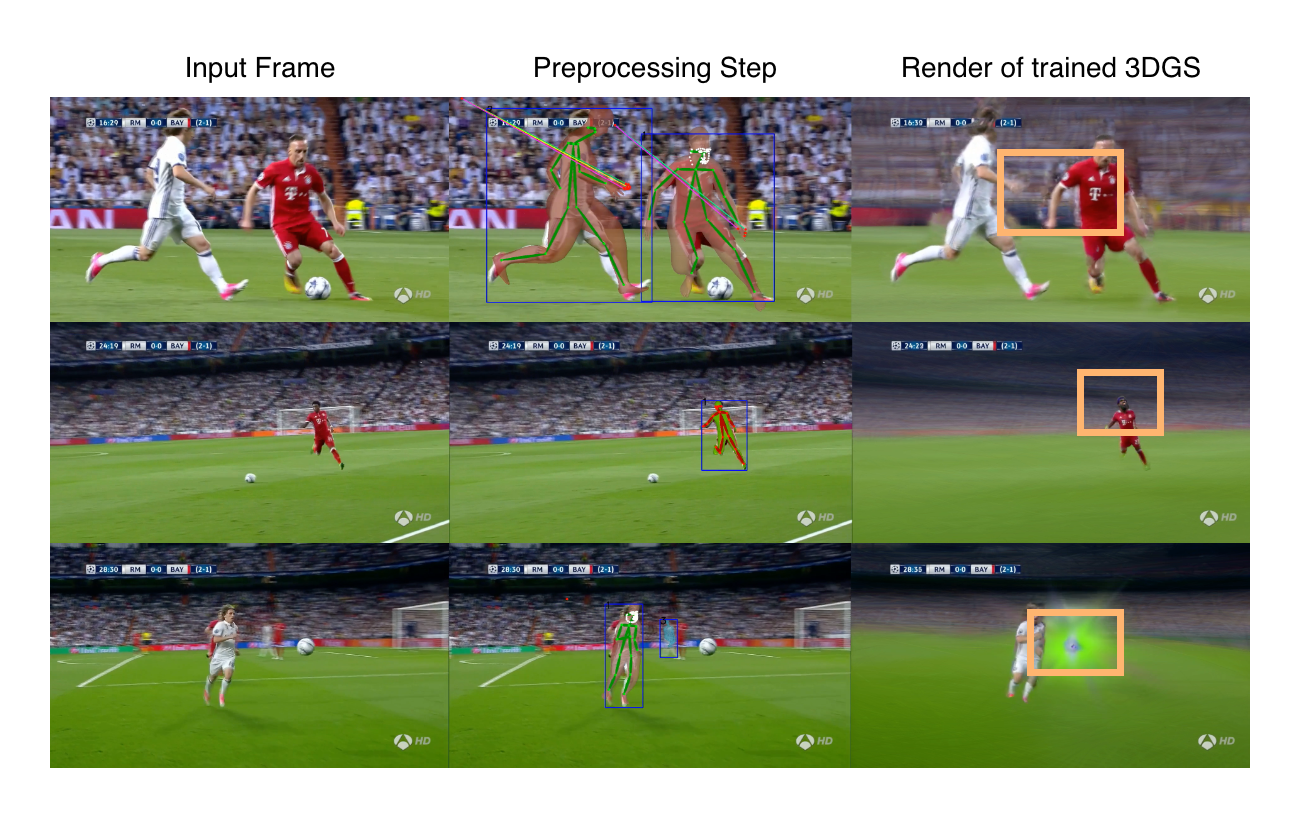
\includegraphics[width=0.8\textwidth]{figures/appendix_gtu_limits.drawio.png}
    \caption{\textbf{Limitations of the Guess the Unseen approach}. We show the input image, preprocessing outputs, and the synthesized training view produced by Guess the Unseen \cite{gtu} on different scenes.}
    \label{fig:appendix_gtu_limits}  
\end{figure}

In contrast to video diffusion methods that aim to directly synthesize a novel-view video, Guess the Unseen (GTU) \cite{gtu} is an optimization-based pipeline that reconstructs a 3D scene representation and then renders novel views from it. Figure~\ref{fig:appendix_gtu_limits} shows qualitative results of GTU on human-centric scenes. The first row highlights a failure mode where imperfect segmentation causes background appearance to leak into the dynamic human model, which leads to artifacts in the synthesized training view. The second row shows distorted facial detail, which we attribute to diffusion-based pseudo supervision producing incorrect high-frequency hallucinations. The last row shows additional artifacts around the ball that are consistent with diffusion-driven hallucinations.


\section{Instance Segmentation}\label{sec:appendix_segmentation}

Instance segmentation is an important preprocessing component in our pipeline because it provides the masks used to separate dynamic humans from the static background. Inaccurate masks can cause background appearance to leak into the supervision signal for the human models, which can introduce artifacts in both reconstruction and rendering.

\paragraph{Experimental setup.} We conducted an initial study that adapts MultiPly's \cite{multiply} progressive mask refinement strategy. Rather than relying only on the initial masks predicted by SAM, MultiPly iteratively reruns SAM during training using improved prompts derived from the current reconstruction. MultiPly also leverages SMPL joints as additional cues. We implemented an analogous refinement loop within our pipeline and evaluated it on Hi4D. In addition, we report results with SAM3 \cite{carion2025sam3segmentconcepts}, which became available during this study and serves as our default mask predictor in the final pipeline.


\subsection{Results}

\begin{table}[!ht]
  \centering
  \small
  \setlength{\tabcolsep}{7pt}
  \begin{tabular}{l
      S[table-format=1.3]
      S[table-format=1.3]
      S[table-format=1.3]}
    \toprule
    \textbf{Method} & \multicolumn{1}{c}{\textbf{IoU} $\uparrow$} & \multicolumn{1}{c}{\textbf{Recall} $\uparrow$} & \multicolumn{1}{c}{\textbf{F1} $\uparrow$} \\
    \midrule
    MultiPly (Init.) & 0.943 & 0.975 & 0.984 \\
    MultiPly (Progressive) & 0.963 & \textbf{0.985} & \textbf{0.990} \\
    Ours (Progressive) & 0.959 & 0.978 &  0.971 \\
    SAM3 & \textbf{0.974} & 0.982 & 0.987 \\
    \bottomrule
  \end{tabular}
  \caption{\textbf{Human instance segmentation results on Hi4D.} Best results are in bold.}
  \label{tab:segmentation_results_hi4d}
\end{table}

\begin{figure}[!ht]
    \centering
    \includegraphics[width=1.0\textwidth]{figures/appendix_prog_sam_limits.drawio.png}
    \caption{\textbf{Prompting strategy for progressive SAM refinement}. The left column shows the prompts given to SAM2, including the mask to refine and a set of positive and negative points. The right column shows the corresponding SAM2 outputs.}
    \label{fig:appendix_prog_sam_limits}  
\end{figure}

Table~\ref{tab:segmentation_results_hi4d} compares our segmentation quality to MultiPly, which reports both its initial masks from SAM1 \cite{sam1} and masks obtained by progressive refinement during training. Our progressive refinement uses SAM2 rather than SAM1. The results show that SAM3 achieves the best IoU and performs competitively in recall and F1, while MultiPly's progressive refinement achieves the best recall and F1. Our adaptation of progressive refinement underperforms both MultiPly's progressive refinement and direct SAM3 segmentation. A likely explanation is that the quality of progressive prompts depends on the underlying reconstruction pipeline that provides the intermediate renderings and silhouette estimates, and our pipeline differs substantially from MultiPly. Overall, these results indicate that using SAM3 directly already provides high-quality masks, which makes additional refinement less critical for our final system.

Figure~\ref{fig:appendix_prog_sam_limits} illustrates our prompting strategy for progressive refinement. In the first row, we prompt SAM2 only once per image and person, which can produce noisy masks. In the second row, we apply an autoregressive strategy that re-prompts the model multiple times, using the refined mask from the previous step as input for the next step. This improves stability in practice, but the resulting masks still fall short of MultiPly's progressive refinement and direct SAM3 segmentation.
